\documentclass{article}
\usepackage[utf8]{inputenc}

%%%%%%%%%%%%%% ADDED BY US %%%%%%%%%%%%%%%%%%%
% \label{ssec:std_pair} \ref{ssec:std_pair}
% https://www.sharelatex.com/learn/Page_size_and_margins
\usepackage[letterpaper, margin=1in]{geometry}
% Inline commenti:::ng


\usepackage[dvipsnames]{xcolor}
% http://latexcolor.com/
\definecolor{navyblue}{rgb}{0.0, 0.0, 0.5}
\newcommand{\rnote}[1]{{\xxnote{SL}{red}{#1}}}
\newcommand{\bnote}[1]{{\xxnote{SL}{blue}{#1}}}
\newcommand{\onote}[1]{{\xxnote{SL}{orange}{#1}}}
\newcommand{\nbnote}[1]{{\xxnote{SL}{navyblue}{#1}}}
\newcommand{\jgnote}[1]{{\xxnote{SL}{JungleGreen}{#1}}}
\newcommand{\bonote}[1]{{\xxnote{SL}{BurntOrange}{#1}}}
\usepackage{amsmath}
% implement conditional notes (turn on/off with \hidenotes above)
\newcommand{\xxnote}[3]{}
\ifx\hidenotes\undefined
  \usepackage{color}
  \renewcommand{\xxnote}[3]{\color{#2}{#1: #3}}
\fi

% Internal section references
\newcommand{\figref}[1]{Fig.\ \ref{#1}}
\newcommand{\secref}[1]{Sec.\ \ref{#1}}
\newcommand{\tabref}[1]{Table \ref{#1}}
\usepackage{moreverb,url}

\usepackage{amssymb}
\let\oldemptyset\emptyset
\let\emptyset\varnothing

\usepackage[utf8]{inputenc}
\usepackage{tikz}
\usetikzlibrary{mindmap}
% Fancier version: http://www.texample.net/tikz/examples/feature/mindmaps/

\usepackage{hyperref}
\hypersetup{
    colorlinks=true,
    linkcolor=blue,
    filecolor=magenta,
    urlcolor=cyan,
}

\usepackage{graphicx}

\usepackage{tikz}
\usetikzlibrary{shapes.geometric, arrows}
\tikzstyle{startstop} = [rectangle, rounded corners, minimum width=3cm, minimum height=1cm,text centered, draw=black, fill=red!30]
\tikzstyle{io} = [trapezium, trapezium left angle=70, trapezium right angle=110, minimum width=3cm, minimum height=1cm, text centered, draw=black, fill=blue!30]
\tikzstyle{process} = [rectangle, minimum width=3cm, minimum height=1cm, text centered, draw=black, fill=orange!30]
\tikzstyle{decision} = [diamond, minimum width=3cm, minimum height=1cm, text centered, draw=black, fill=green!30]
\tikzstyle{arrow} = [thick,->,>=stealth]


\usepackage{natbib}
\usepackage{graphicx}

% for subfigure
\usepackage[font=footnotesize]{subcaption}
\usepackage[font=footnotesize]{caption}

% Font
\usepackage{lmodern}        % Latin Modern family of fonts. Very much like Computer Modern, but with many more glyphs
                            % (e.g., for characters with accents, glyphs, cedillas, etc)
\usepackage[T1]{fontenc}    % fontenc is oriented to output, that is, what fonts to use for printing characters.
                            % http://tex.stackexchange.com/questions/44694/fontenc-vs-inputenc
                            % http://tex.stackexchange.com/questions/664/why-should-i-use-usepackaget1fontenc

                            %%%%     FONTS PACKAGE OPTIONS in the Preamble  %
%%%%     always replace default Computer Modern with Latin Modern [T1] encoding:
\renewcommand{\ttdefault}{lmtt} % MONO Latin Modern Font % T1 encoding of cmtt font style
\renewcommand{\rmdefault}{lmr} % SERIF Latin Modern Font % T1 encoding of cmr font style
\renewcommand{\sfdefault}{lmss} % SANS Latin Modern Font % T1 encoding of cmss font style
% switch to sans family and then choose a font from the family
\renewcommand{\familydefault}{\sfdefault}
%  %  %   %   %   %   %   %   %   %   %   %   %   %   %   %
%  %  % PSNFSS \ssfamily fonts (SANS)
% \usepackage{helvet} % PSNFSS Font, in every TeX distribution
% \usepackage{avant}  % PSNFSS Font, in every TeX distribution
%  %  % Extended \ssfamily (Sans) fonts; load extraFonts option from TeX
\usepackage[scaled=0.88]{berasans}% package has a handy scaling option
% \usepackage{libris}   % a nice, almost handwritten calligraphic look
% \usepackage{biolinum} % included with the {Libertine} font package
% \usepackage{iwona}
% \usepackage{paratype}
%%%  END OF SANS SERIF FONT PACKAGES
%  %  %  %   %   %   %   %   %   %   %   %   %   %   %   %   %   %
%  %  % PSNFSS \rmfamily fonts (SERIF)
% \usepackage{mathptmx}  % Times % PSNFSS Font, in every TeX distribution %
% \usepackage{charter}   % Bitstream Charter % PSNFSS Font, in every TeX distribution %
% \usepackage{mathpazo}  % Palatino % PSNFSS Font, in every TeX distribution
% \usepackage{bookman}   % Bookman % PSNFSS Font in every TeX
% \usepackage{chancery}  % Zapf Chancery % PSNFSS Font in every TeX, a Calligraphic Font
% \usepackage{newcent}   % New Century Schoolbook % PSNFSS Font in every TeX distribution % To replace it's Avant Garde sans add this:% \renewcommand{\sfdefault}{xxx}
%  %  % Extended \rmfamily (SERIF) fonts; load extraFonts option from TeX
% \usepackage[scaled=0.88]{beraserif}% package has a handy scaling option
% \usepackage{XCharter} % Bitstream's Charter extended with many style varieties
% \usepackage{fouriernc}% Century Schoolbook % compact and lighter than New Century Schoolbook
% \usepackage{tgschola} % TeX Gyre Schola, New Century Schoolbook with many font style varieties
% \usepackage{tgtermes} % TeX Gyre Termes, Times with many font style varieties
% \usepackage{tgbonum}  % TeX Gyre Bonum, Bookman with many font style varieties
% \usepackage{tgpagella}% TeX Gyre Pagello, a Palatino font with many font style varieties
\usepackage{fourier}  % Utopia, package {utopia} is obsolete
% \usepackage{txfonts}  % TX Serif and Sans (Helvetica)
% \usepackage{kpfonts}  % KP Serif and Sans, large variety of font styles
% \usepackage{libertine}% Libertine + Linux Biolinum (Extra TeXLive fonts)
% \usepackage{fbb}      % A Garamond Font (Bembo) with many font styles
% \usepackage[varg, cmintegrals, cmbraces, ]{newtxtext,newtxmath}  % Other options: libertine, uprightGreek (U.S.) or slantedGreek (ISO), etc...
% \usepackage{tgtermes}                                            % Only serif ("TeX-Gyre" text)
% \usepackage{kpfonts}                                             % "Kepler" fonts
% \usepackage{mathpazo}                                            % Based on Hermann Zapf's Palatino font
% \usepackage{txfonts}                                             % More than a decade old
% \usepackage{pslatex}                                             % Obsolete?
% \usepackage{mathptmx}
% \usepackage[scaled=.90]{helvet}
% \usepackage{courier}
%%% END SERIF FONTS
%%% NOTE!!! Be sure to comment out all but ONE Serif and ONE Sans
%%% from the package selections above.
%  %  %   %   %   %   %   %   %   %   %   %   %   %   %
%  %  %   %   %   %   %   %   %   %   %   %   %   %   %
%  %  % Load Math Support if necessary
%
% \usepackage[myFontPackage]{mathdesign}
%
%
%%% END OF FONTS In the Preamble
%%%%%%%%%%%%%%%%%%%%%%%%%%

% http://stackoverflow.com/questions/741985/latex-source-code-listing-like-in-professional-books
\usepackage{listings}
\lstset{
language=C,
basicstyle=\footnotesize\ttfamily,
numbers=left,
numberstyle=\tiny,
frame=tb,
columns=fullflexible,
showstringspaces=false
}

% https://contrarymotion.net/2007/03/23/latex-itemize-bullet-characters/comment-page-1/
% http://tex.stackexchange.com/questions/36443/how-to-change-the-nested-itemize-bullet-characters
\usepackage{enumitem}
\setlist[itemize,1]{label={$\circ$}}
\setlist[itemize,2]{label={$\diamondsuit$}}
\setlist[itemize,3]{label={$\star$}}
\setlist[itemize,4]{label={$\rightarrow$}}
\setlist[itemize,5]{label={$\ast$}}
\setlist[itemize,6]{label={$\cdot$}}


\DeclareMathOperator*{\argmin}{arg\,min}
\DeclareMathOperator*{\argmax}{arg\,max}

\begin{document}
% this is an alternate method of creating a title
%\hfill\vbox{\hbox{Gius, Mark}
%       \hbox{Cpe 456, Section 01}  
%       \hbox{Lab 1}    
%       \hbox{\today}}\par
%
%\bigskip
%\centerline{\Large\bf Lab 1: Security Audit}\par
%\bigskip
\title{Roots and humans teaming up in pursuit-evasion games: modeling and learning issues}
\author{Shen Li}

\maketitle

% !TEX root = ./root.tex
\section{Introduction}
\subsection{Pursuit-evasion Game}
\subsubsection{Game}
\begin{itemize}
    \item World = undirected graph with exits
    \item Pursuers and evaders take turns to act
    \begin{itemize}
        \item Pursuers move at the same time triggered by human
        \begin{itemize}
            \item Human pursuer has an imprecise model of the world
            \item Robot pursuer adapts it $\pi^*$ for the non-optimality of its human teammate
        \end{itemize}
        \item Robot evaders move at the same time rationally
    \end{itemize}
    \item Robot evaders will be removed when they cannot move except stepping onto a pursuer or evader
        \begin{figure}[ht]
            \centering
            \begin{subfigure}[b]{.5\linewidth}
            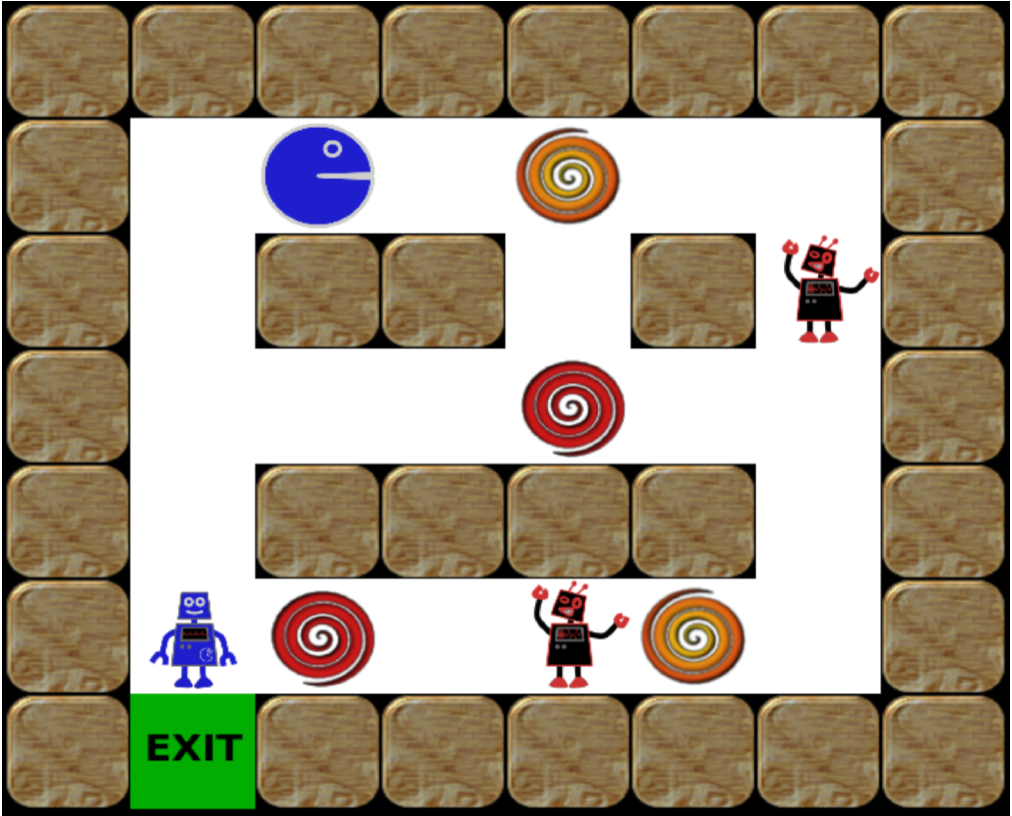
\includegraphics[width=\linewidth]{./game.png}
            \caption{}
            \end{subfigure}
            \caption{The pursuit-evasion game (agents can be teleported through swirls)}
            \label{fig:game}
        \end{figure}
    \bnote{so evaders have to be cornered before removed? Yes! It has to be cornered by other pursuers or evaders}
\end{itemize}

\subsubsection{Challenges}
\begin{itemize}
    \item It is hard for 1 human and 1 robot to predict each other's behavior
    \item It is harder for multiple humans and multiple robots to predict each other's behavior
    \item Simplification: more pursuers than evaders and robot pursuers cannot capture all the evaders without human help
    \item \bnote{Future work: we can model the fact that the human will also try to interpret and adapt to the robots' behaviors. And also we can model if human trusts his robot teammates or not.}
\end{itemize}

\subsubsection{Motivation}
\begin{itemize}
    \item Investigate how a robot can account for human teammates and adapt
\end{itemize}
\subsubsection{Related Work}
\begin{itemize}
    \item Bounded memory model for table carrying task in \figref{fig:bam} (\cite{Nikolaidis_2016_8035}).
        \begin{figure}[ht]
            \centering
            \begin{subfigure}[b]{.5\linewidth}
            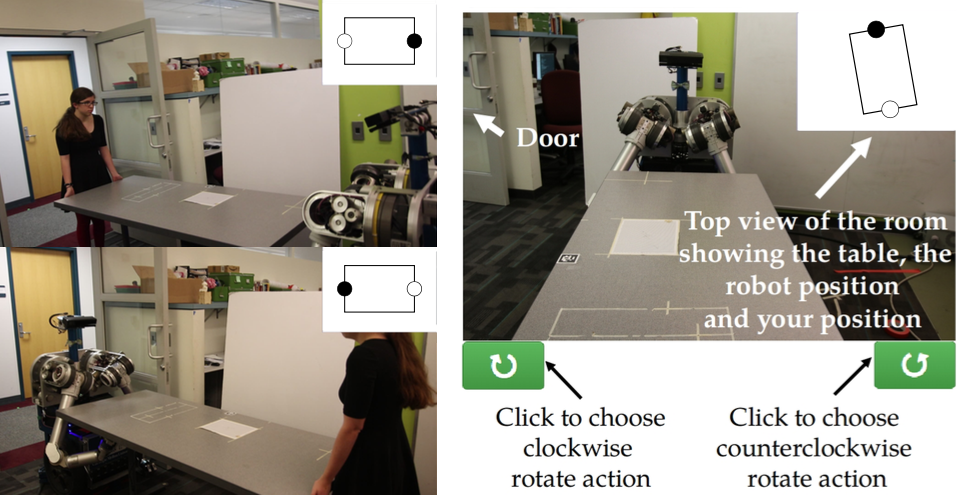
\includegraphics[width=\linewidth]{./bam1.png}
            \caption{}
            \label{fig:bam1}
            \end{subfigure}
            \begin{subfigure}[b]{.4\linewidth}
            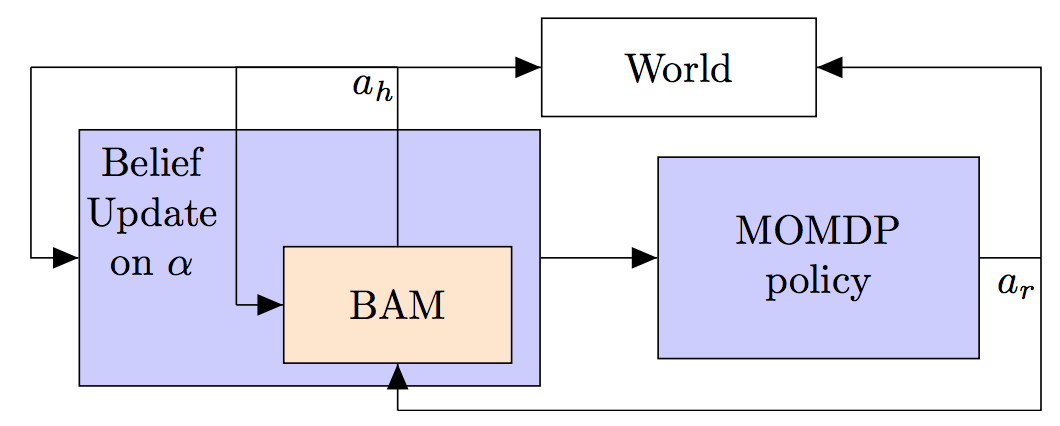
\includegraphics[width=\linewidth]{./bam2.png}
            \caption{}
            \label{fig:bam2}
            \end{subfigure}
            \caption{In \subref{fig:bam1}, the one on the left is the human-robot table carrying task. Rotating the table so that the robot is facing the door (top, Goal 1) is better than the other direction (bottom, Goal 2), since the exit is included in the robot’s field of view and the robot can avoid collisions. The one on the right is the UI with instructions. In \subref{fig:bam2}, Integration of BAM into MOMDP formulation.}
            \label{fig:bam}
        \end{figure}
    \item Cross training \figref{fig:cross_train} (\cite{nikolaidis2013human}).
        \begin{figure}[ht]
            \centering
            \begin{subfigure}[b]{.5\linewidth}
            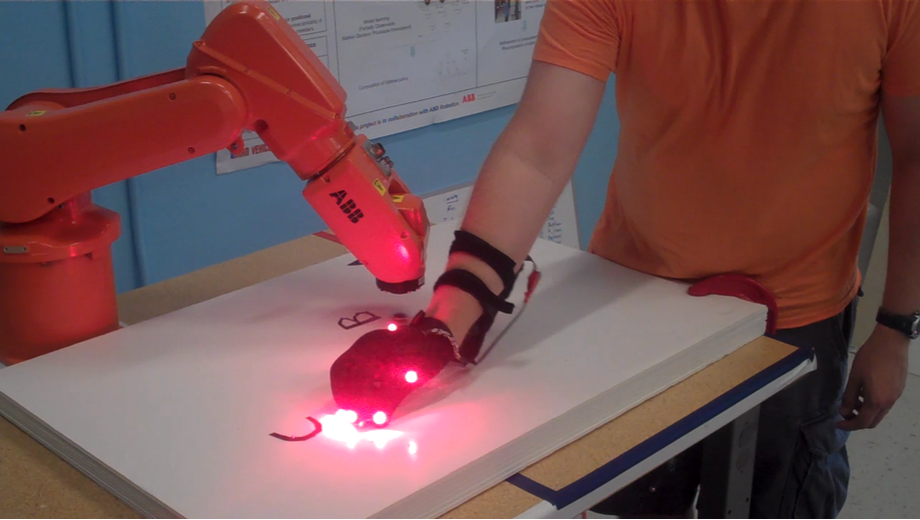
\includegraphics[width=\linewidth]{./cross_train.png}
            \caption{}
            \end{subfigure}
            \caption{In \subref{fig:bam1}, }
            \label{fig:cross_train}
        \end{figure}
    \item my project on when to intervene
\end{itemize}

\subsubsection{Contribution}
\begin{itemize}
    \item Usually people have to use reinforcement learning to train a robot model used for this particular person, which requires lots of data before start. We want the game to play at start. We need to learn the parameters on-line quickly to get a team policy.
    \item We have a problem.\\
    $\Rightarrow$ What model we use?\\
    $\Rightarrow$ How to take into account that human acts optimally based on limit information? Human less capable $\Leftrightarrow$ more random in the transition function of human action\\
    $\Rightarrow$ What parameters we want to use to shape the model in real time based on the human input?\\
    $\Rightarrow$ We can make the robot act optimally, but optimality means making the best decision \textbf{based on the current state}. Not the absolute best decision in all time.\\
    $\Rightarrow$ This is very expensive computationally so we have to do approximation, which will make robot pursuers suboptimal\\
    $\Rightarrow$ How to deal with robot pursuers suboptimality vs human suboptimality?
    \item A trust model of human
    \item \bnote{applications? see the last section}
    \item \bnote{Future work
        \begin{itemize}
            \item Does explanations, demonstrations, or hints help to make collaboration more fluent?
            \item Now we are enabling robots to collaborate with people and adapt to people, but we can also make people adapt to robots. The robots have to assist people when only people, not the robots, can capture the evaders. So the robots will give explanations, demonstrations, or hints to change human behaviors so that people can follow optimal policy computed by the robots. In which way the people can follow the commands from the robots? In natural language or demonstrations?
            \item The reason why the robots cannot just give orders to the people about what to do is that robots and people are better at different things. For example, robots are better at computing but people are better at heuristics. How to make them do what they are good in collaboration?
        \end{itemize}
        }
\end{itemize}

\subsubsection{Assumptions}
\begin{itemize}
    \item Full knowledge: all agents know all agents' positions
    \item The number of people and robots are fixed\\
    \bnote{Future work: we can relax it? Randomly adding new members or removing members}
    \item Centralized control\\
    \bnote{Future work: distributed?}
    \item Evaders do not cooperate and acting based on a fixed policy to minimize the pursuers' reward\\
    \bnote{Future work: human + robots vs human + robots. We can also collect data about how people play against people without robots.}
    \item \bnote{How to make sure human can win (winning strategy)?}
\end{itemize}


\subsubsection{MDP}
\begin{itemize}
    \item Human $h \in H$, robot pursuer $p \in P$, robot evader $e \in E$
    \item $s_h \in S_H, s_p \in S_P, s_e \in S_E$
    \item $\forall x \in H+P+E,\:A(s_x) = N(v(s_x))$ - neighbor of occupied vertices of $x$ (deterministic)
    \item $R_{shared} = \text{shared by } \forall p \in P,h \in H \propto \frac{\text{number of captured evaders}}{\text{number of steps } p,h \text{ have taken}}$\\
    \\
    \bnote{common reward for pursuers and single MDP for each evader}
    \item $\forall x \in H+P+E,\:T(s_{x,t+1}|s_{x,t},a_{x,t}) \leftarrow Pr(s_{x,t+1}|s_{x,t},a_{x,t}) \leftarrow \{s_{x',t} \:\:|\:\: \forall x' \in H+P+E\:\:s.t.\:\:x' \neq x\}$
    \item $\forall e \in E$ (semi-deterministic) 
    \begingroup
        \addtolength{\jot}{1em}
        \begin{align*}
            A^*(s_e) = 
            \begin{cases}
                \text{move\_away} & \forall x \in H+P, ||s_e-s_x|| < \epsilon\\
                \argmin_{a \in A(s_e)} R_{shared} & \text{otherwise}
            \end{cases}
        \end{align*}
    \endgroup
    \bnote{1 - maximize the distance to that particular pursuer? Yes}\\
    \bnote{2 - minimize the total reward of all the pursuers? Each evader has its own MDP}
    \item $\forall p \in P$ (deterministic)\\
    $A^*(s_p) = \argmax_{a \in A(s_p)} R_{shared}$\\\\
    \bnote{each agent acts based on the latest state? Not on other agents' actions? Yes! trying to be optimal based on the current state}\\
    \bnote{Would the pursuers and the evaders lock each other and no one is gonna win??? No! because the evaders never cooperate. So each of them will have a single MDP to make the optimal decisions. But the pursuers are sharing 1 single big MDP to make the optimal decisions together, which means that they cooperate. Human is also part of the pursuer model.}
    \item Discounted\\
    \rnote{why?}
    \item Steps
    \begin{enumerate}
        \item Robot pursuers compute the evader actions based on optimality (you can pre-compute their optimal actions), or locally optimal, or some simple heuristic (e.g. the evaders will go random or greedy or $\epsilon-greedy$ to maximize the distance to pursuers)
        \item Robot pursuers update the transition function (probability distribution) for the human
        \item After taking into account the randomness introduced by the human (flatten the probability distribution) and those fixed evader actions, we can do value iteration or some approximation to compute the optimal policy in the big MDP shared by all pursuers.
        \item At the same time, each robot evader will compute optimal action based on its single MDP and execute.
        \item We can learn some parameters and how to represent human ability
    \end{enumerate}
\end{itemize}



\subsubsection{Human Model}
\begin{itemize}
    \item Human ability value prior $\Leftarrow$ human input
    \begin{itemize}
        \item ability to discriminate among choices = difficulty of the decision $\Leftarrow$ $||a_h||$
        \item ability to look ahead = ability to foresee the impacts of decisions $\Leftarrow$ $min(\text{number of turns before a capture})$
        \item ability to grasp useful knowledge about the current state = $Q_h(s,a)$ $\Leftarrow$ $s_{x,t} \forall x \in H+P+E$
        \item \bnote{ability to understand the robot teammates' reasonings = look back in the past}
        \item \bnote{trust or confidence on robot teammates' ability to win the game}
    \end{itemize}
    \bnote{Do we assume these abilities? Do we have to prove them from some psychological literatures? Or are these 3 abilities parts of our contributions? We have to get them from literatures about how to model human ability in playing these games!}

    \item update $Pr(s_{h,t+1} | s_{h,t}, a_h)$
    \begin{enumerate}
        \item update trust $\tau$
        \item $Pr(s_{h,t+1} | s_{h,t}, a_h) \leftarrow \text{normalize}(Q(s_{h,t}, a_h))$
        \item smooth $Pr(s_{h,t+1} | s_{h,t}, a_h)$ based on $||a_h||$\\
        The more actions, the harder to make choice, the smoother the probability distribution will be.
        \bnote{this is flattening the probability distribution in the transition function to be uniform, which will increase the entropy}
        \item Distance to go = $\tau_{DTG} = min(\text{number of turns before a capture}) \leftarrow \text{optimal human MDP}$
        \item Look ahead $\tau_{LA} = \text{number of steps the system thinks the human can predict}$
    \end{enumerate}
    \rnote{???????}
\end{itemize}

\rnote{human swarm interaction people?}


\subsubsection{Applications}
\begin{itemize}
    \item We can evaluate our model by compare our prediction about what human will do and what human really do. If it is getting closer and closer as the human keeps playing the game, we are good.
\end{itemize}

\subsubsection{Applications}
\begin{itemize}
    \item In reality, the game will be amazing to study how human play with robots in real time.
    \item Specific application
    \begin{itemize}
        \item This is a task where 1 person and multiple robots are chasing multiple robots. We can apply this directly to scenarios like 1 policeman and multiple robot cars chasing criminals.
    \end{itemize}
    \item Looking at it from a bigger picture
    \begin{itemize}
        \item Multiple evaders = multiple goals in this task
        \begin{itemize}
            \item It is harder than \cite{Nikolaidis_2016_8035} because we have multiple goals because it \bnote{involve some task planning to choose goals}
            \item It could be used in the table-clearing task where 1 person and multiple robots are collaborating in removing multiple objects from the table
        \end{itemize}

        \item Evaders are moving = the goals are changing in a dynamic environment
        \begin{itemize}
            \item It is harder than table-clearing task because the objects on the table are not moving.
            \item It is more like the real situation where you have to \bnote{adapt your goal} to the current situation dynamically every time after you achieve a sub-goal because the situation might have changed after you achieve this sub-goal.
        \end{itemize}

        \item Evaders are escaping from pursuers = there are distractions naturally in the task so the task is even harder and the game is more interesting.
        \begin{itemize}
            \item \bnote{This makes the collaboration between human and multiple robots necessary to finish the task}
        \end{itemize}

        \item Task = multiple human collaborate with multiple robots in finishing multiple goals which are changing all the time.
        \item We can also verify the abilities of different evaders and different robot pursuers.
        \begin{itemize}
            \item All the robots have the same ability, but some are good and some are bad.
            \item All the robots have different abilities. Some are good at chasing or running (speed $\times$ 2), while the others are good at capturing ($Pr(\text{successful\_capturing})$ is higher).
            \item Human and robot are good at different things. How do we leverage that? What human abilities and what robot abilities work together more efficiently?
        \end{itemize}

        \item More questions to ask
        \begin{itemize}
            \item Human-robot collaboration strategy - split or not?
            \begin{itemize}
                \item Rule: whenever a pursuer touches an evader, the evader will be removed.
                \item Question to ask: do human-robot team focus on 1 target at the same time to corner it make sure it will never run away or split to chase different targets?
            \end{itemize}
            \item Task switching
            \begin{itemize}
                \item Rule: The evader will be removed only when all the human and robot pursuers circle the evaders so that the evader has no way to go.
                \item Question to ask: human and robot will first focus on 1 target. When do they decide to switch a target because the first target is escaping efficiently?
            \end{itemize}
            \item Dynamic vs static?
            \item Multiple people/robot pursuers/evaders or not?
        \end{itemize}
    \end{itemize}
\end{itemize}










\bibliographystyle{plain}
\bibliography{references}
\end{document}




